\documentclass[a4paper,10pt, twocolumn]{article}

\usepackage[utf8x]{inputenc}
\usepackage{amssymb,amsmath}
\usepackage{graphicx}
\usepackage[italian]{babel}
\usepackage{hyperref}
% \usepackage{mathtools}
\usepackage{amssymb,amsmath}

\title{Relazione al progetto: \\ Naruto Hand Seals Fighting\\ del corso di\\Sistemi e Applicazioni
Multimediali}
\author{Michele Tamburini \\ mtamburi@cs.unibo.it}
\makeindex

\begin{document}

\maketitle

\section{Abstract}
Il progetto nasce con lo scopo di esplorare uno dei campi della \emph{Augmented Reality}, che
prevede l'uso delle mani nell'interazione uomo-macchina.
La realizzazione ultima consiste di un gioco di combattimento in modalità "picchiaduro"
che prende ambientazione e scenografia dall'ormai noto anime giapponese "Naruto".
Le mosse per così dire speciali, dovranno essere attivate non con semplici
combinazioni di tasti, ma attraverso le posizioni ed i gesti delle mani dell'utente,
acquisiti attraverso una webcam, che saranno poi analizzati da un motore di
riconoscimento per verificarne l'accuratezza.
L'implementazione del presente prevede il 
motore di riconoscimento e una semplice sezione di addestramento
per l'utente, che lo coinvolga nell'apprendimento di alcune mosse.\\
Vengono utilizzate librerie \emph{OpenCV} per l'analisi delle immagini, 
\emph{Guichan} per l'interfaccia grafica, \emph{SDL} ed il linguaggio C++.

\section{Stato dell'arte}
La ricerca di tecniche che favoriscano metodologie di utilizzo dei calcolatori
attraverso forme di interazione sempre pi\'{u} innovative, quali ad esempio
l'uso del proprio corpo, ha aperto la strada gi\'{a} da qualche tempo
a nuove sfide per il mondo informatico.\\
Il campo di ricerca dell'\emph{``hand tracking''} vuole dare all'utilizzatore
del calcolatore la possibilit\'{a} di un controllo, completo o parziale, di questo,
attraverso i complicati movimenti o stimoli che la mano umana \'{e} in grado di fornire.
L'acquisione di questi, sia essa agevolata dall'ausiglio di sensori particolari,
guanti o addirittura con la mano nuda, risulta essere la prima problematica da affrontare,
comune a tutte le proposte fino ad ora osservate (\cite{handTrackHCI} \cite{handTrackNoMarkers}
 \cite{handNavigator} \cite{hugeSurvey} \cite{mitGlove}. 
 Gli spunti proposti nella bibliografia, lontano
dall'essere esaustiva sull'argomento, vogliono semplicemente offrire una panoramica ad ampio
spettro di alcune soluzioni a tale problema.

\section{Progetto: introduzione}
  \subsection{Ambientazione}
  L'ormai celeberrimo anime ``Naruto'' ha portato anche in Italia una storia di fanstasia
  dalle forti connotazioni orientali. Tra gli ingredienti maggiormente apprezzati dal
  grande pubblico risiede il fatto che i personaggi utilizzano movimenti 
  delle mani estremamente complicati per lanciare mosse di arti marziali speciali.
  Ognuna di queste \`{e} composta da un numero variabile di ``sigilli'' (posizioni degli arti
  superiori) che corrispondo ai 12 segni zodiacali cinesi.\\
  Nel seguente progetto ho inserito tutti e soli tali gesti, ovvero non si tengono in considerazione
  movimenti diversi (come il battito delle mani) che pur compaiono nell'anime.
  Lo scopo del giocatore sar\`{a} quello di riprodurre
  alcune posisioni che vedr\`{a} raffigurate sottoforma di immagini. Ciascuna
  di queste \`{e} denominata segno, o sigillo (signs, seals). Una mossa (Move) \`{e} dunque
  costituita da un numero variabile di segni presi tra i 12 sopra descritti.
  
  \subsection{Il nostro problema nel dettaglio}
  In questo lavoro non ho certo la pretesa di affrontare un tema cos\'{i} imponente come 
  quello dell'hand tracking. Il problema si riduce infatti ad una analisi di immagini
  seppur non priva di compromessi e difficolt\`{a}. A differenza di alcuni lavori
  di spicco che usano un database e oggetti esterni
  per l'inferenza della reale posizione della mano \cite{mitGlove}, in questo caso non
  \`{e} necessario avere una precisa cognizione del punto di partenza e di 
  fine dell'arto.
  Il giocatore \`{e} libero di eseguire qualunque movimento e, una volta pronto,
  aziona l'acquisione del gesto, che si traduce per il calcolatore con: l'acquisizione 
  di alcuni frame di immagine, trasformazione di questi con tecniche di processazione
  dell'immagine e confronto con un template precedentemente preparato.\\
  Un punto che abbatte notevolmente la dimensione del problema, ed evita quindi l'uso 
  di un database, si basa proprio su una carattestica derivata dall'ambientazione:
  sebbene le combinazioni che possono avere luogo siano infinite (permutazioni di 12 
  elementi di lunghezza arbitraria) i diversi gesti da riconoscere rimangono comunque 12.
  
  \subsection{Pensando in grande}
  Fondamentalmente questo gioco risiede nella categoria ``picchiaduro''.
  L'ingrediente della \emph{Augmented Reality} emerge nel
  momento in cui l'utente abbandona la tastiera per interagire con le proprie mani 
  attraverso la webcam ed eseguire dal vivo i gesti necessari per la mossa selezionata.\\
  Per ciascuno gli verr\`{a} notificato il livello di accuratezza 
  calcolato in una scala da 0 a 100.
  Al termine dell'ultimo viene poi restituito il voto medio.
  
%  \subsection{Goal Oriented Design}
%  In questa sezione introduco in maniera assolutamente superficiale ed approssimata 
%  alcune linee guida per il personaggio principale e quello secondario pi\`{u} rilevante.\\
%  Tale citazione ha solo lo scopo di fornire una migliore rappresentazione di uno scenario 
%  di utilizzo dell'applicazione.
%  \begin{itemize}
%   \item[Principale] Lela, donna sulla quarantina, sposata e madre di Gioacchino. 
%   Ha un impiego presso un'impresa 
%  \end{itemize}


\section{Introduzione alla Libreria OpenCV}
OpenCV \`{e} una libreria per l'analisi delle immagini estremamente versatile e completa.
Nonostante la mia completa ignoranza a riguardo, mi sono convito a sfruttarla fin 
dalle fasi di studio di fattibilit\`{a} del progetto, 
spinto sia dal suggerimento avuto dalle lezioni del corso di 
Sistemi e Applicazioni Multimediali \cite{slide} che dall'innumerevole ammontare di 
commenti positivi reperibili dalla rete.\\
Sono necessarie solo poche nozioni per prendere dimestichezza con questa. 
Prima fra tutte la gerarchia delle strutture dati (CvArr, CvMat), ed 
in particolare quella usata per la memorizzazione dell'immagine:
IplImage. Quindi l'uso delle principali funzioni di analisi delle 
immagini: cominciando con l'applicazione dei filtri basilari (Laplaciano,
Sobel, di Smoothing...) per arrivare al dominio delle frequenze, 
rilevazione dei contorni, utilizzo della webcam (o addirittura multi-cam). 
Estremamente apprezzabile \`{e} la possibilit\`{a} di un
approccio ``lazy'', per usare un termine informatico. In un certo senso \`{e} possibile
iniziare la fase di programmazione senza preoccuparsi dell'uso preciso di una 
determinata funzione, utilizzandola dapprima con impostazioni di default,
per poi scendere nei dettagli solo in un secondo momento.\\
Altro pregio della libreria \`{e} la facilit\`{a} della visualizzazione del risultato
grafico a schermo (attraverso le funzioni cvNamedWindow(), cvShowImage()) che
consentono una veloce analisi del risultato delle operazione all'interno di
ogni singola parte del progetto.\\
Bisogna osservare tuttavia che, sebbene i primi capitoli del manuale ``Learning
OpenCV'' \cite{opencvOReally},
collocato probabilmente tra i pi\`{u} consigliati nella rete, siano davvero utili 
per approcciarsi alla libreria, lo stesso non si possa dire delle sezioni pi\`{u}
specifiche, che non sostituiscono un libro di testo per l'analisi delle immagini.
Durante tutto il periodo di sviluppo risulta per\`{o} necessario armarsi del 
manuale ufficiale \cite{opencvReference}, disponibile anche online.\\
Un secondo punto a favore di tale libreria \`{e} la reperibilit\`{a} di numerosi 
frammenti di codice ed esempi che si possono trovare in rete, ma che chiaramente
vanno affrontati con la giusta ponderazione prima di essere utilizzati nel
proprio lavoro.
  
  
\section{Descrizione del progetto}
Questa sezione contiene la descrizione della parte centrale del lavoro svolto.

  \subsection{Sezione di Acquisizione} 
  Con il termine acquisione ho inteso la cattura di frames attraverso la webcam.
  Webcam pensata integrata all'interno del pc portatile, anche se nulla esclude 
  l'utilizzo di un dispositivo diverso, purch\`{e} riconosciuto dal sistema, e
  impostato per essere quello di default.\\
  L'oggetto Camera si compone semplicemente di una
  classe in grado di inizializzare una struttura di tipo Capture (della libreria OpenCV),
  e sfruttarla per reperire un immagine di tipo IplImage*. Su questa avranno quindi
  luogo la fase di processazione e valutazione della macchina di riconoscimento
  (vedi di seguito).	
  
  \subsection{Logica di Gioco}
  Per consentire lo sviluppo di un'applicazione che mostri i connotati per una stesura 
  pressoch\'{e}  completa, 
  \`{e} necessario immergerla nello scenario dell'ambientazione almeno dal punto 
  di vista logico. Ho volutamente evitato tediosi dettagli, come ad esempio l'occorrenza nella
  storia
  di una particolare mossa o il personaggio che l'ha effettuata per la prima volta,
  che rendono magari
  l'anime estremamente interessante, 
  %in particolare per un personaggio secondario  tremendamente esigente, 
  ma che ai fini dell'attuale
  lavoro non sono poi cos\`{i} rilevanti.\\
  Tuttavia ciascuna mossa viene catalogata in base al proprio tipo, rango di difficolt\`{a} e 
  livello, in maniera il pi\`{u} possibile fedele all'anime. Per un compito cos\`{i}
  strutturato mi sono affidato alla versalitit\`{a} del linguaggio XML, e l'uso della libreria
  ``TinyXML'' \cite{tinyXml} per la sua manipolazione. Grazie a questi accorgimenti 
  risulter\`{a} forse pi\`{u} agevole l'espansione del codice in futuro.\\
  A questo si \`{e} poi aggiunto un forte apporto ingegneristico per rendere fin dal 
  principio tale sezione manutenibile senza troppi sforzi.
  In figura \ref{gameLogicDiagram} \`{e} riportato il diagramma UML della logica di gioco.
   
  \subsection{Stack di Gioco}
  Non \`{e} difficile osservare come questa sezione, 
  cos\`{i} come pure l'interfaccia grafica, non sono state l'oggetto di cure maniacali.
  In particolare ho voluto create strutture architetturalmente valide che dessero il
  massimo riuso di codice, ma allo stesso tempo sufficientemente versatili in termini
  di espandibilit\`{a}.\\
  Il risultato di tali ragionamenti \`{e} sintetizzato dal diagramma \ref{gameStackDiagram}.
  La macchina di gioco (\textit{GameMachine}) altro non \`{e} che un semplice contenitore di
  elementi, come ad esempio i menu o la sezione di addestramento (\textit{TrainingSection}), 
  ciascuno dei quali deve provvedere la funzione che ricoprir\`{a} il ruolo di 
  ciclo principale. Infatti la GameMachine dispone tutti i moduli contenuti in una 
  struttura a stack ed eseguir\`{a} sempre la funzione di quello in cima.\\
  A ciascuno di questi, sia esso un menu, o un modulo differente, viene 
  affidato un controller, che deve essere in grado di gestire eventi 
  conformi all'interfaccia SDL.
    
  \subsection{L'interfaccia Grafica}
  Ciascun elemento di gioco (\textit{GameElement}) ha la necessit\`{a} di mostrastri all'utente
  attraverso un'interfaccia grafica. La libreria Guichan \cite{guichan} mi \`{e}
  sembrato il compromesso migliore tra quelle che erano
  le potenzialit\`{a} utili a ricoprire le richieste grafiche, tutt'altro che esigenti,
  e compatibilit\`{a} con le librerie nativamente previste per il progetto.
  Questa si trova perfettamente compatibilie con SDL. Il punto di contatto tra 
  OpenCV, per l'acquisizione delle immagini dalla webcam, e l'integrazione con 
  la sezione grafica \`{e} reso possibile grazie alla convesione dall'immagine 
  IplImage di OpenCV alla superficie SDL (SDL\_Surface) e quindi alla visualizzazione
  tramite l'opportuno oggetto Guichan. Il risultato del procedimento \`{e}
  quanto mostrato dal punto 2 di figura \ref{screenshot}.
  
  \begin{figure}
  %\centering
    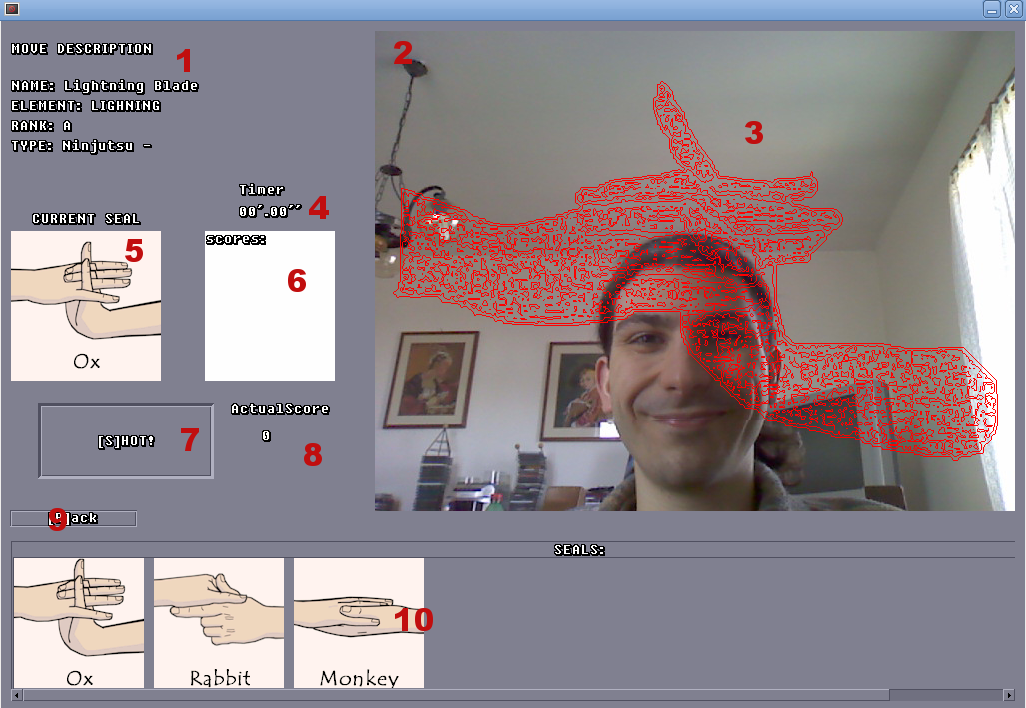
\includegraphics[scale=0.25]{screenShot}
    \caption{Screenshot dell'applicazione durante una esecuzione}
  \label{screenshot}       
  \end{figure}
  
  Di seguito elenco le sezioni della finestra, mostrata in \ref{screenshot},
  descrivendole brevemente:
  \begin{enumerate}
   \item descrizione della mossa: oltre al nome vengono visualizzate anche il tipo,
	 il grado di difficolt\`{a} (non di esecuzione) ed il nome reale giapponese;
   \item schermo che mostra l'immagine acquisita istantaneamente attraverso la webcam;
   \item sono la traccia della corretta posizione delle mani e delle dita: pi\`{u} il
	 giocatore riuscir\`{a} ad esservi fedele e migliore sar\`{a} il punteggio ottenuto;
   \item timer: appena premuto il pulsante ``Shot!'' (o usata la relativa abbreviazione),
	 viene attivato un cronometro di 3 secondi per dare modo al giocatore di 
	 riposizionarsi correttamente;
   \item mostra la posizione delle mani per eseguire il sigillo attuale;
   \item contiene la lista dei punteggi ottenuti per ciacun sigillo fino al momento attuale;
   \item \`{e} il pulsante che attiva il cronometro e quindi la fase di acquisizione;
   \item mostra in tempo reale il punteggio che si otterrebbe nel caso scattasse l'acquisione;
   \item pulsante che retrocede al menu della lista delle mosse per la selezione di una nuova;
   \item sigilli necessari al compimento della mossa attuale.
  \end{enumerate}

\begin{figure*}[tp]
  \centering
    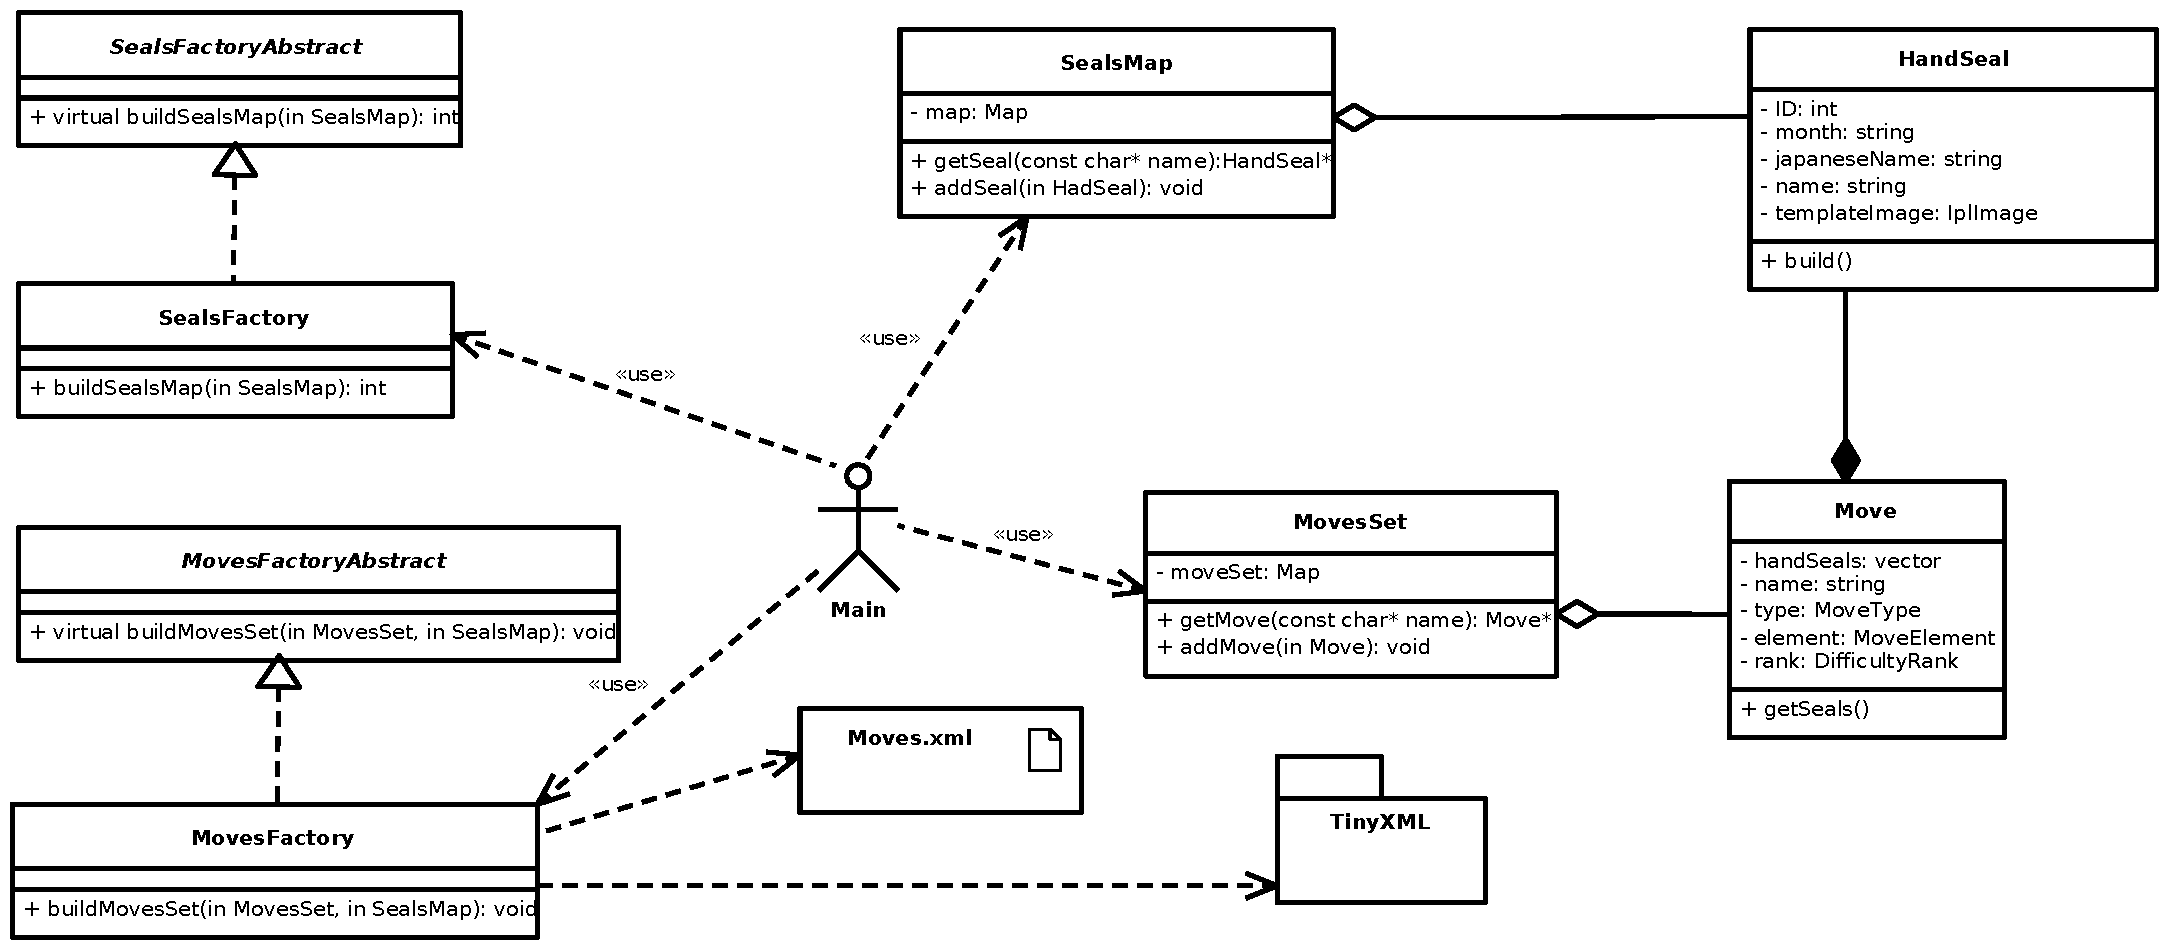
\includegraphics[scale=0.45]{UmlDiagrams/gameLogic.pdf}
    \caption{Uml diagram of the GameLogic section.}
  \label{gameLogicDiagram}       
  \end{figure*}
  
  \begin{figure*}[bp]
  \centering
    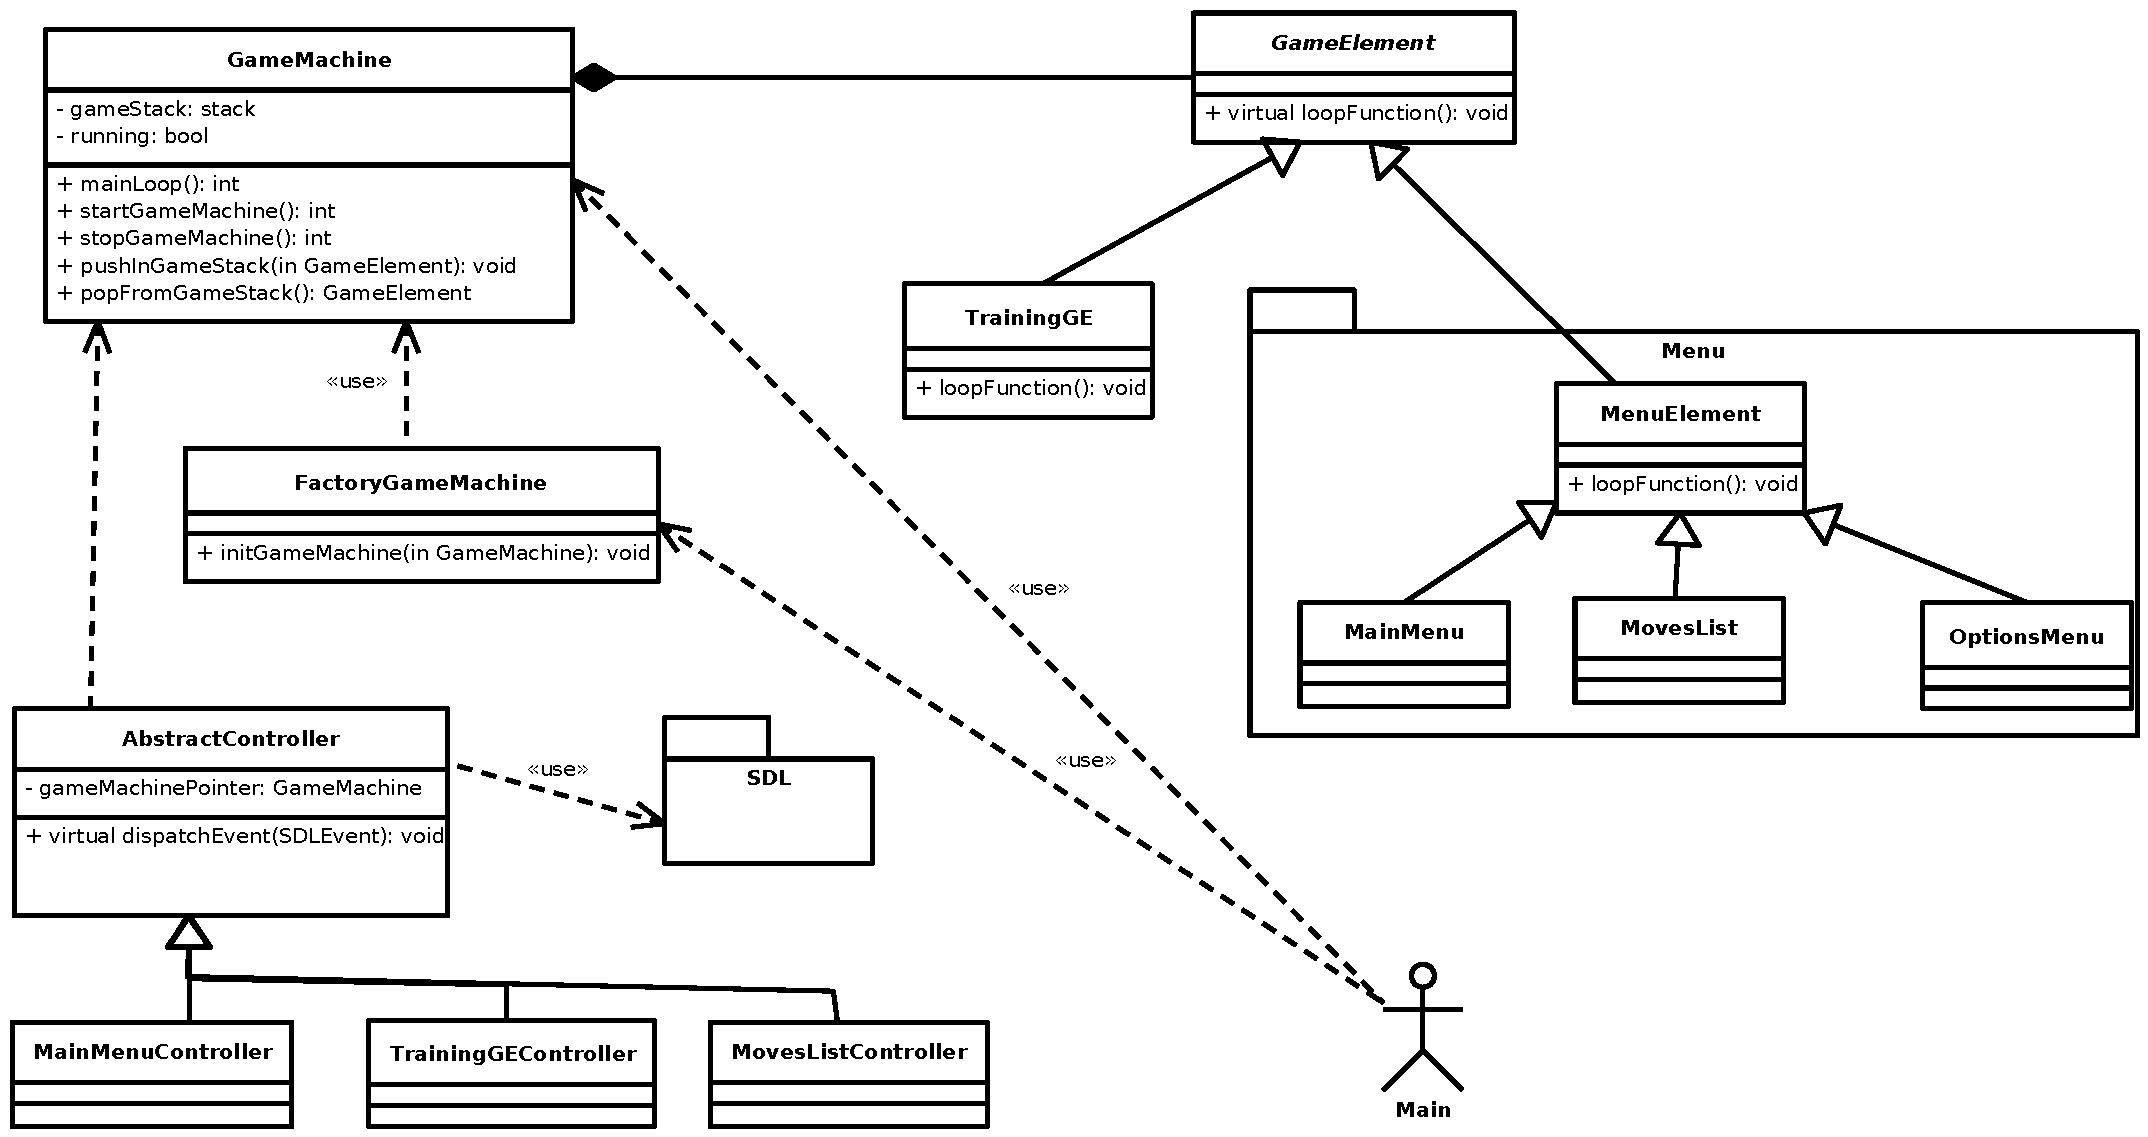
\includegraphics[scale=0.4]{UmlDiagrams/gameStack.pdf}
    \caption{Uml diagram of the GameStack section.}
  \label{gameStackDiagram}       
  \end{figure*}

\section{Riconoscimento}
Il cuore del progetto \`{e} costituito dalla macchina di riconoscimento del gesto effettuato.
Come gi\`{a} accennato la qui presente soluzione applica combinazioni di 
semplici tecniche di analisi delle immagini.\\
Per quanto riguarda la realizzazione della sezione di riconoscimento, 
fin dalla primordiale idea, ho voluto mantenere un approccio il pi\`{u} possibile modulare
e versatile ai cambiamenti, in modo da poter poi provare agevolmente diverse metodologie
di elaborazione. La macchina corrisponde ad un contenitore di moduli, ciascuno 
dei quali esegue una ben precisa operazione sull'immagine.\\
Il settaggio completo completo di questa prevede: la scelta dei moduli
da inserirvi ovvero la strategia, una funzione per il processing ed una per la 
valutazione.
Una volta applicato questo, se si volesse scendere
%Tutto il procedimento, dall'avvio fino alla valutazione, si pu\`{o} suddividere in
%3 frasi: caricamento dei moduli, processazione (\textit{Processing Phase}), valutazione
%(\textit{Evaluation Phase}).\\
nel dettaglio di ogni singolo passo per 
ogni frame il si osserverebbe un procedimento che consiste nel:
\begin{itemize}
 \item acquisire il frame attraverso la webcam, 
 \item richiamare la funzione di \textbf{processing} della macchina di riconoscimento,
 \item sfruttare poi la funzione di \textbf{valutazione} fornendo come parametri
 il risultato della fase precedente ed il template di riferimento
 per il sigillo corrente,
 \item raccogliere il risultato ottenuto.
\end{itemize}
I \textbf{template}, di cui si \`{e} parlato anche in precedenza,
corrispondo alle immagini dei sigilli prive di sfondo o
forme di rumore, processate attraverso una particolare strategia e sfruttate
quindi dalla funzione di valutazione. Nella sezione \textit{Template Creation} 
si trova infatti l'occorrente a questo scopo: lanciando lo
script che vi si trova vengono convertite le immagini orginali ``grezze'' 
in template e poste nella directory di destinazione dalla quale si lancer\`{a}
l'eseguibile. \\
\`{E} bene tenere a fianco il diagramma di figura \ref{recognitionEngineDiagram} 
per avere chiare le diverse parti di questa sezione.
 
  \begin{figure*}[tp]
     \centering
    %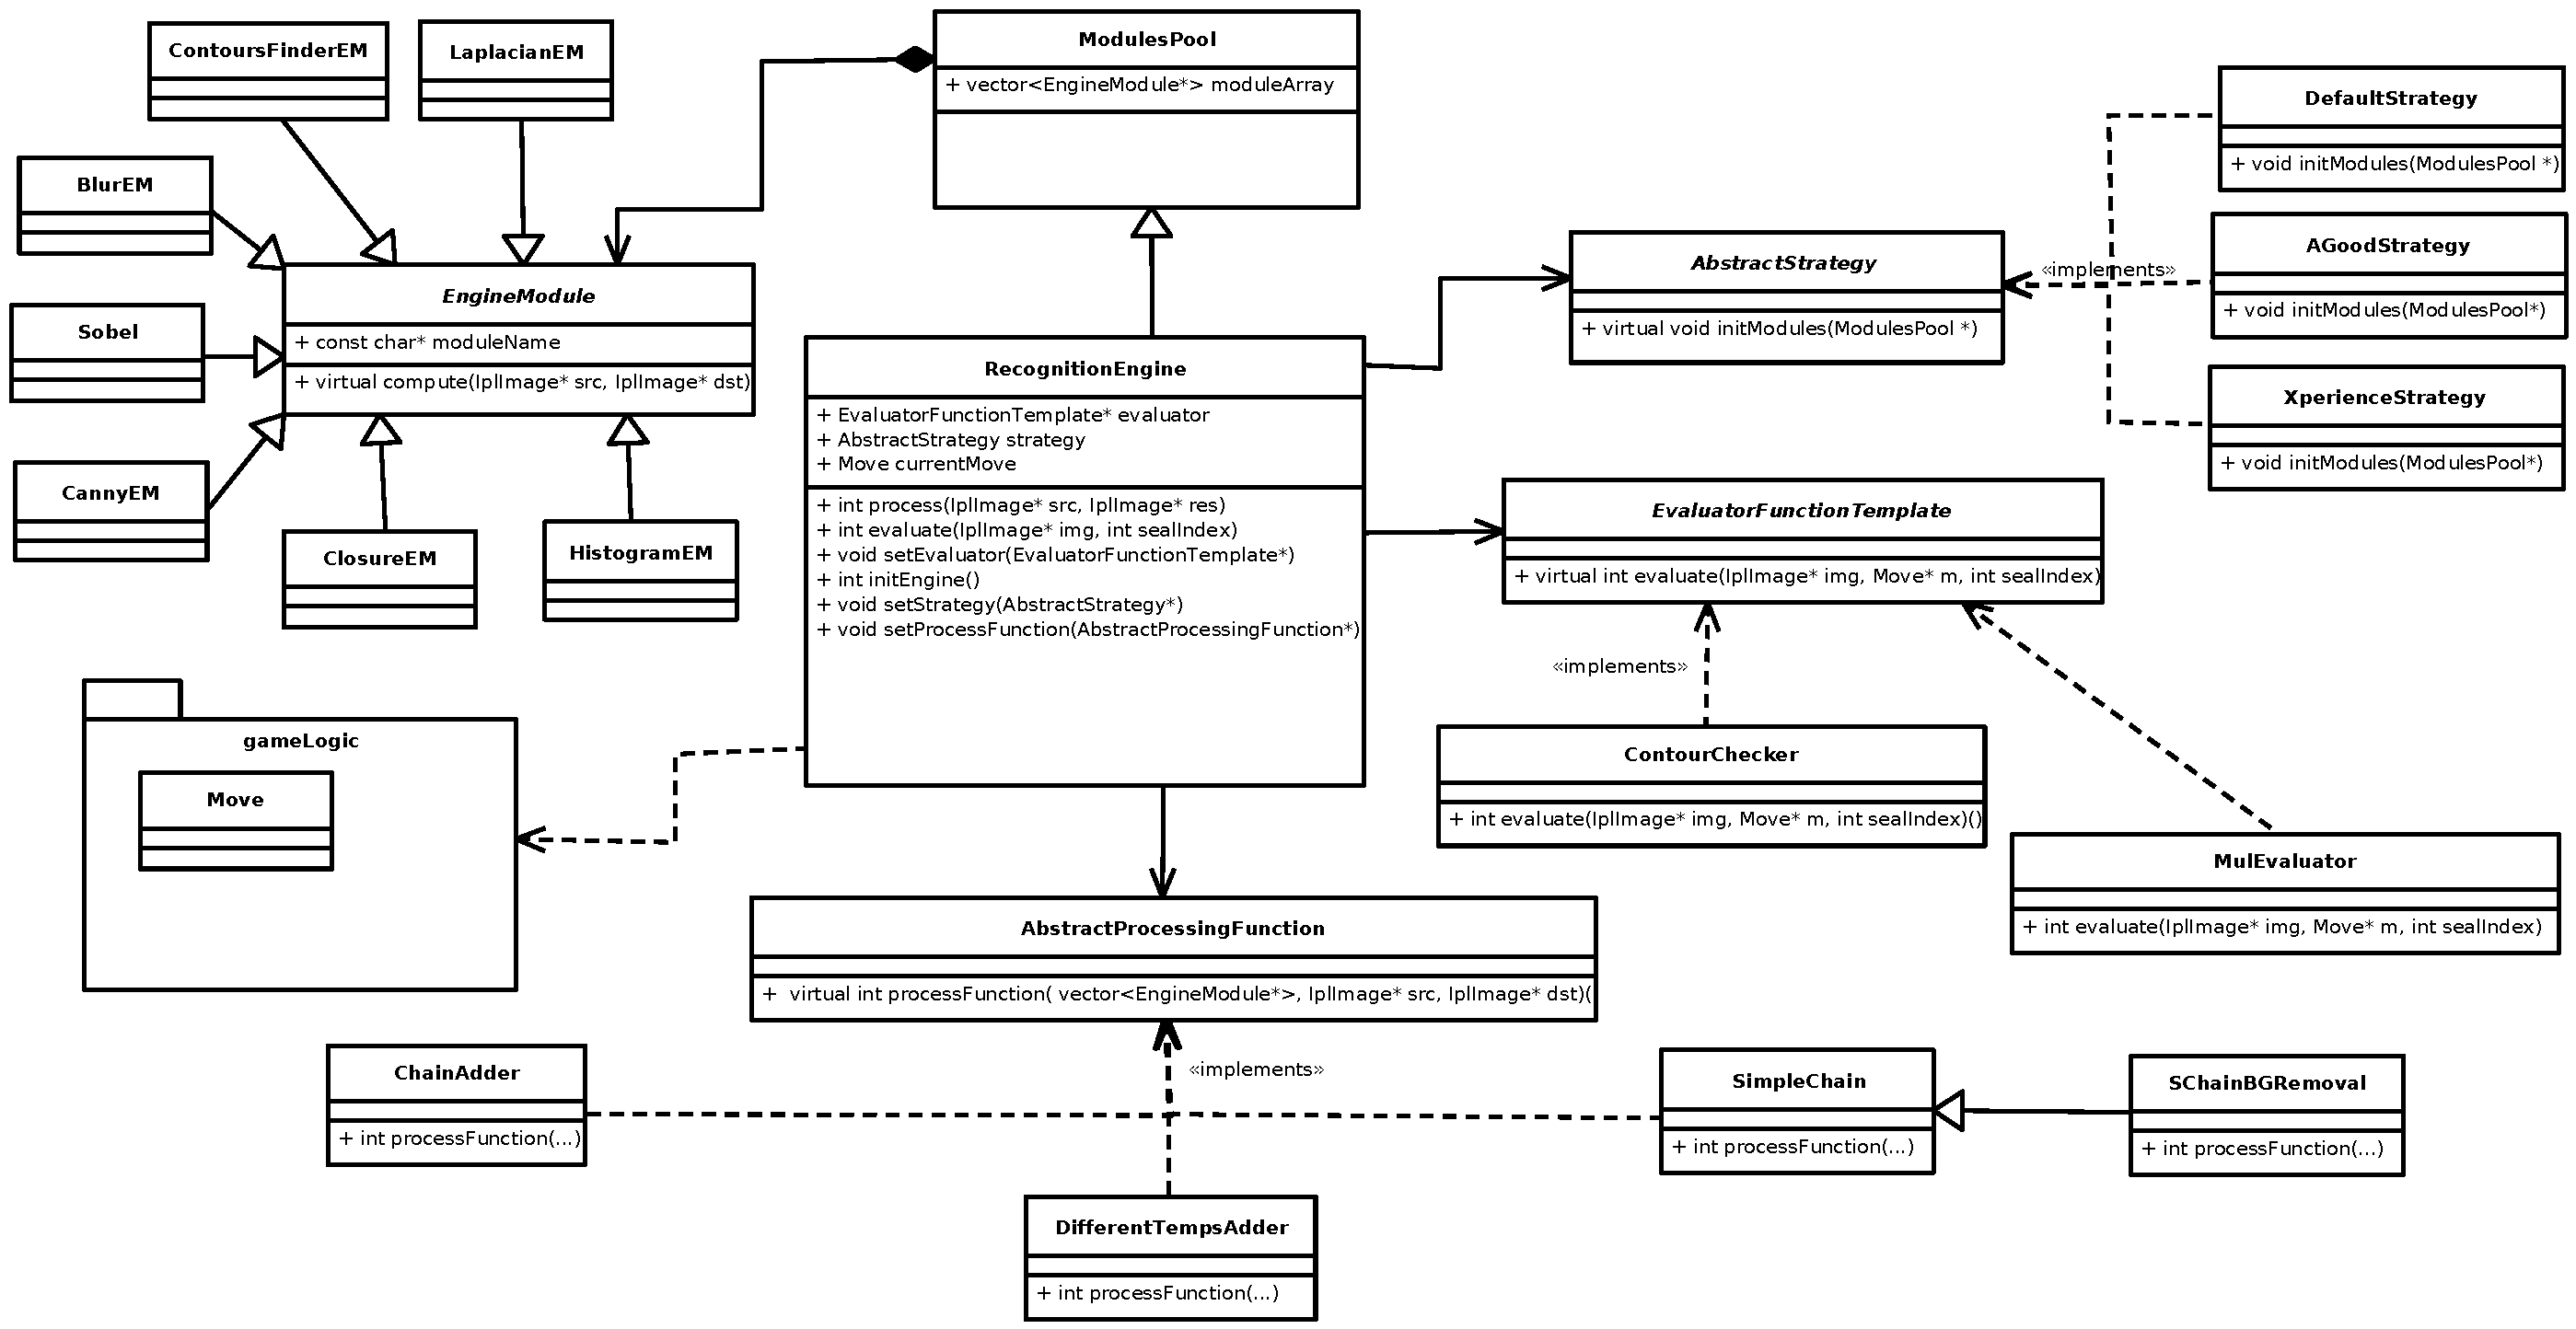
\includegraphics[angle=90, scale=0.328]{UmlDiagrams/recognitionEngine.pdf}
    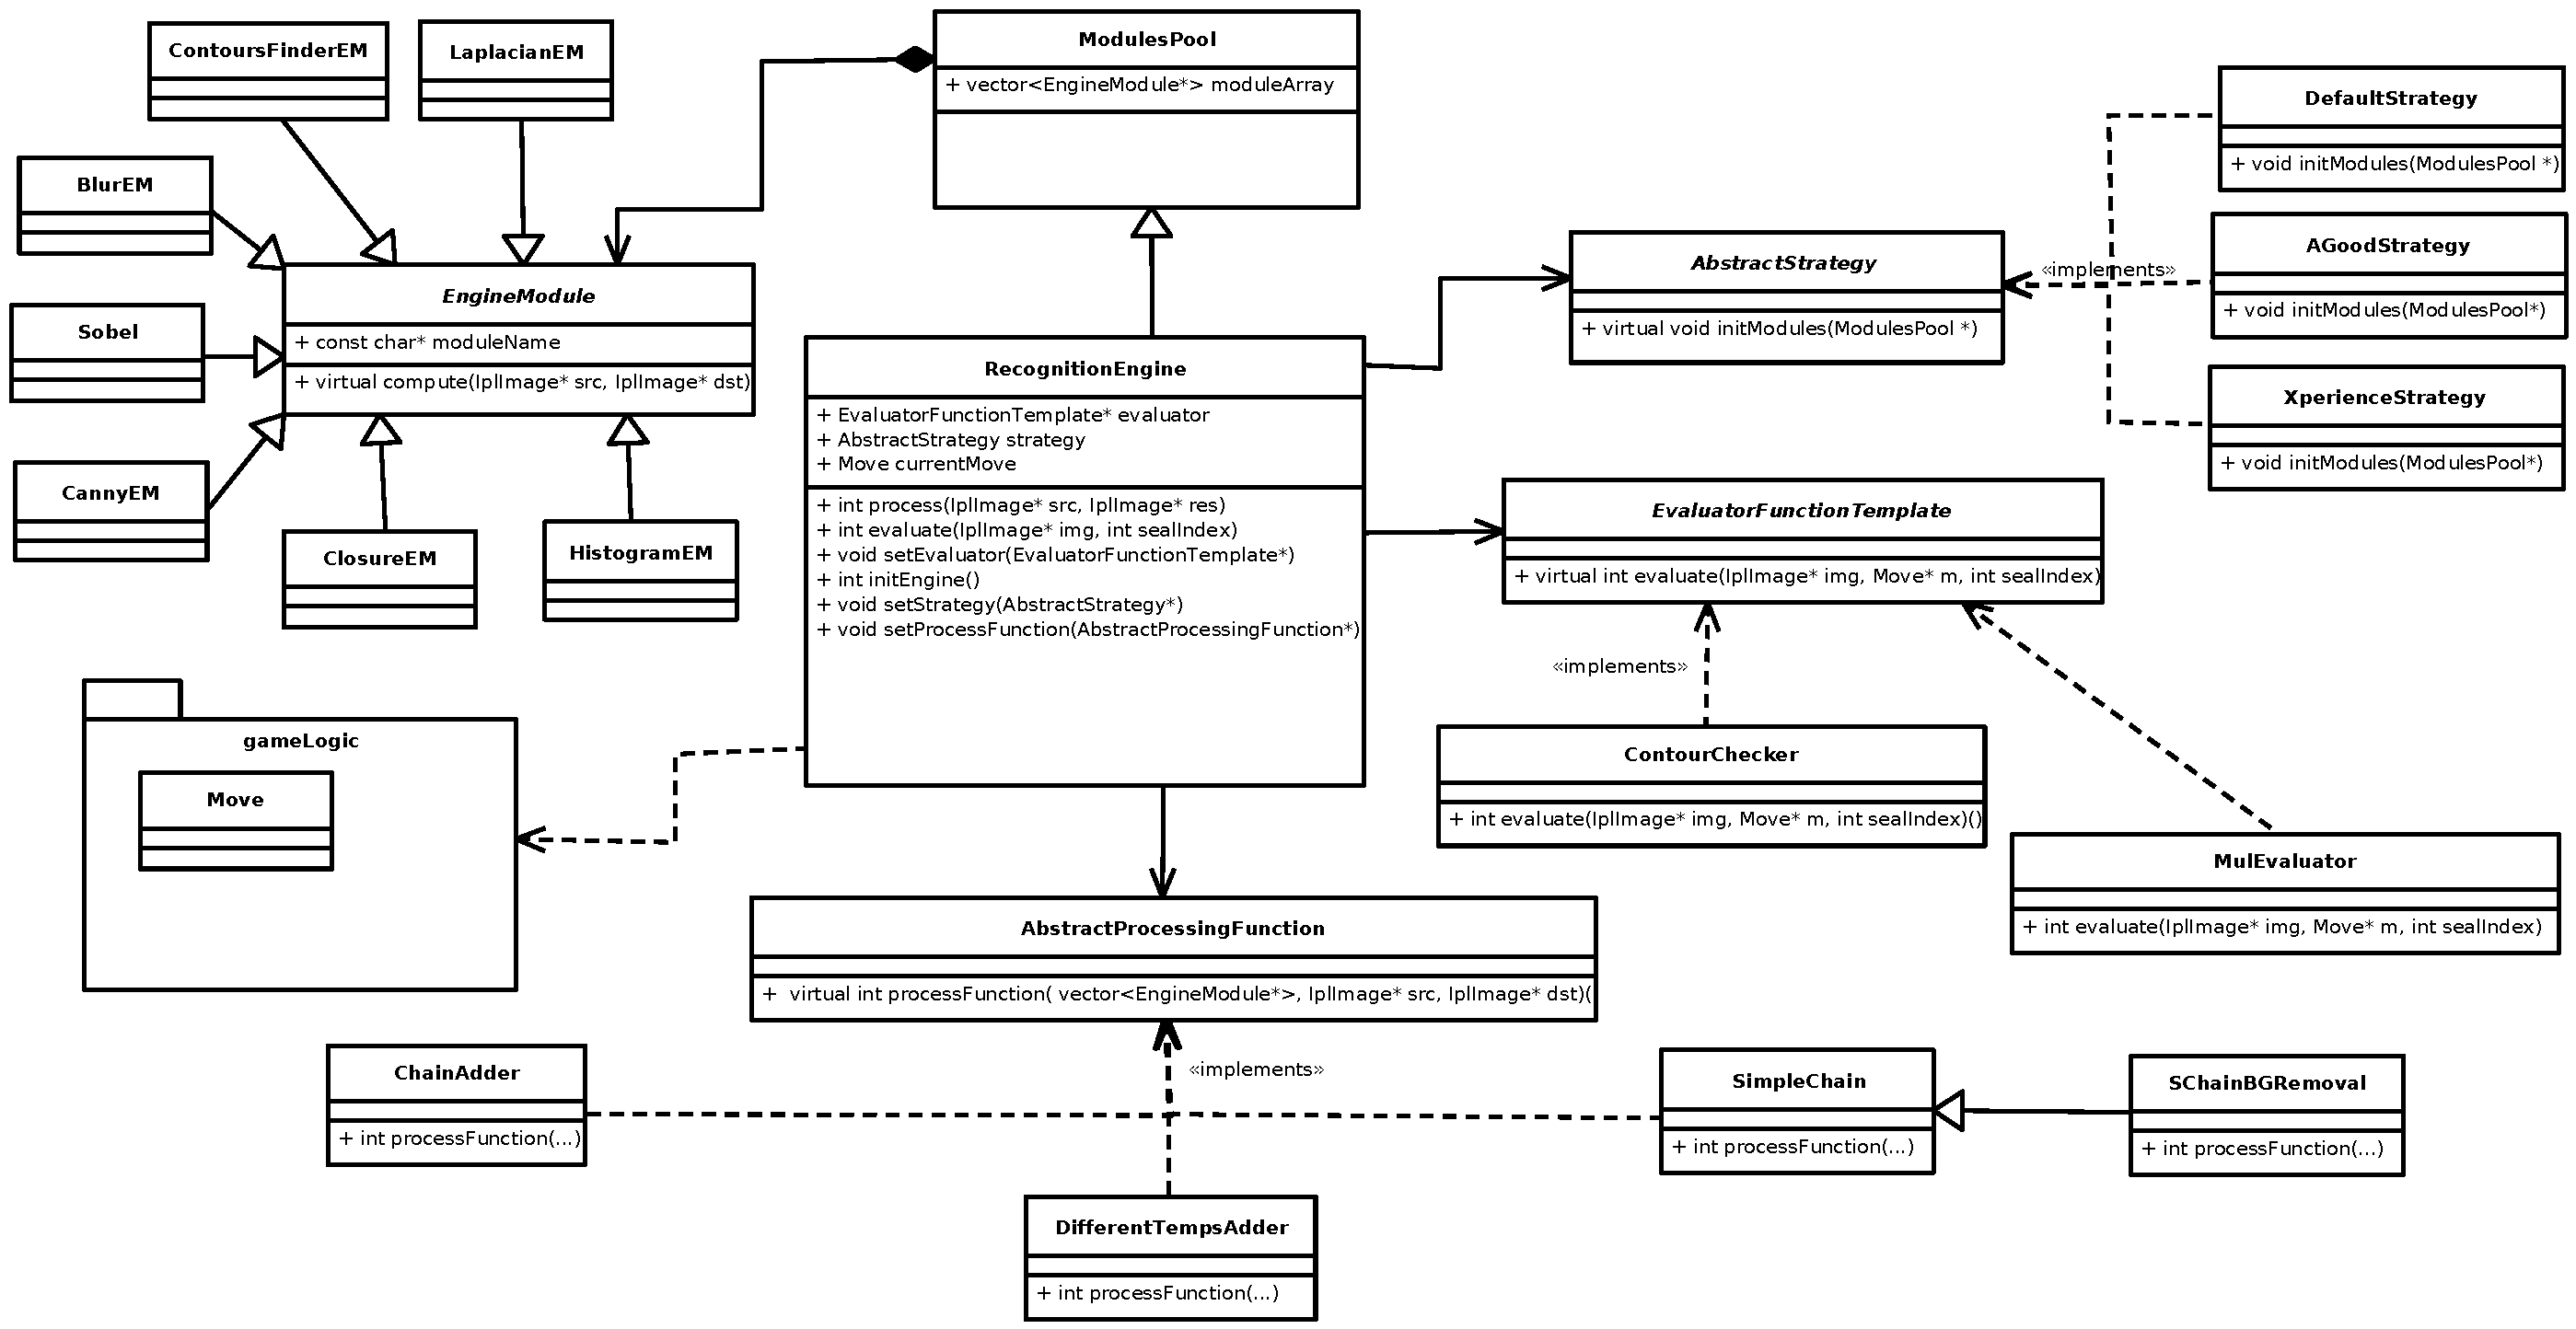
\includegraphics[angle=90, scale=0.5]{UmlDiagrams/recognitionEngine.pdf}
    \caption{Uml diagram of the Recognition Engine Section.}
    \label{recognitionEngineDiagram}
  \end{figure*}

  \subsection{Moduli e Strategie}
  %alcuni moduli più importanti
  %l'ordine dei moduli è rilevante
  Indicher\`{o}
  con il termine \textbf{Modulo} una classe ereditata da \textit{EngineModule} 
  che implementa la funzione
  
  \begin{center}
    \begin{verbatim}
    int compute(const IplImage* src, 
		      IplImage* dst)
    \end{verbatim}
  \end{center}
   e pu\`{o} quindi essere aggiunta nell'insieme dei moduli (\textit{ModulesPool})
  della macchina di riconoscimento.
  L'implementazione di questa dovr\`{a} prevedere dunque l'azione di processing, 
  per la quale il modulo stesso 
  \`{e} pensato, sull'immagine in ingresso src, e la restituzione del risultato in dst.
  Bisogna tener presente che \`{e} rilevante la posizione di ciascun modulo.
  %l'ordine di inserimento dei moduli. 
  Dal momento che l'unit\`{a} di dialogo tra questi sono le immagini, dunque matrici
  di pixel, l'applicazione in ordine diverso di filtri o altre operazioni quali l'estrazione
  dei contorni, pu\`{o} condurre a risultati estremamente diversi. Un esempio canonico
  riguarda il filtro di smoothing posto in genere sempre prima di un operatore Laplaciano.\\
  Un \textbf{strategia} invece definisce quali moduli inserire nel bacino della macchina,
  in che ordine, e con quali carattestiche. Ciascuna classe appartenente alla gerarchia
  che si estende dalla classe \textit{AbstractStrategy}, adempie a questo compito. 
  
  \subsection{Rimozione dello sfondo}
  Un modulo di estrema importanza \`{e} quello della rimozione dello sfondo.
  La capacit\`{a} di individuazione delle forme viene fortemente condizionata
  dalla situazione luminosa della stanza e dalla complessit\`{a} 
  e dal numero di oggetti presenti alle spalle del giocatore.
  Con complessit\`{a} si intendono sia la forma stessa che le caratteristiche 
  riflessive (superfici lucide o opache).\\
  Per fare un esempio che aiuti alla comprensione ritorniamo per un istante
  allo scenario mostrato dalla camera in figura \ref{screenshot}.
  Le fonti luminose di forte intensit\`{a} sono tra le peggiori 
  cause di rumore. Nel lampadario posto alle spalle del giocatore sono poste
  due lampadine a basso consumo a luce bianca: esso rappresenta un ottimo esempio
  di disturbo dell'acquisizione se testato di sera e con luci accese.
  Un ulteoriore esempio, che porta facilmente a falsi positivi,
  \`{e} rappresentato dai due quadri posti sul muro: essi spiccano senza alcuna
  difficolt\`{a} nell'analisi di rilevazione dei contorni, in particolare 
  se vi si aggiunge il fatto che tendono a riflettere buona parte dei
  raggi di luce che li colpiscono (vedi angolo inferiore del quadro 
  a destra).\\
  La rimozione dello sfondo adottata sfrutta un principio di facile intuizione: 
  prevede cio\`{e} l'acquisizione di alcuni frame,
  utili a catturare le parti fisse della scena,
  prima della fase di gioco, momento in cui il giocatore
  posiziona e muove le mani. Il modello di sfondo proposto fa poi uso 
  della statistica e si individuano la media e la correlazione 
  delle immagini catturate.\\
  Sia $p(x,y)$ un'immagine, si calcolano: 
  \begin{equation}
  S(x,y) = \sum_{f=1}^{N} p(x,y) 
  \end{equation} 
  
  \begin{equation}
  Sq(x,y) = \sum_{f=1}^{N} p(x,y)^2 
  \end{equation}   
  dove $f=frame$ e $N=$ \textit{numero totale di frame}.
  
  Dunque la media sar\`{a}:  
  \begin{equation}
   M(x,y) = \dfrac{S(x,y)}{N}
  \end{equation}
  
  e la deviazione standard:
  \begin{equation}
   \sigma(x,y) = \sqrt{ \dfrac{Sq(x,y)}{N} - M(x,y)^2}
  \end{equation}
  
  Questo definisce il nostro modello per la rilevazione degli 
  oggetti fissi nella scena. Data una immagine acquisita in un secondo 
  momento si pu\`{o} sfruttare la quantit\`{a} appena ricavata per dividere
  gli elementi in primo piano da quelli sullo sfondo con 
  la seguente procedura.\\
  Sia $P(x,y)$ la nuova immagine acquisita, allora:
  
  \begin{equation}
   | M(x,y) - P(x,y) | \leq \lambda \sigma(x,y)
  \end{equation}
  
  dunque:
  \begin{center}
  $  
   | M(x,y) - P(x,y) |^2 \leq (\lambda \sigma(x,y))^2
    \newline
    \newline
   | M(x,y) - P(x,y) |^2 \leq \lambda^2 \sigma(x,y)^2   
  $ 
  \newline
  
  \end{center}
  dove $\sigma(x,y)^2$ \`{e}:  
  \begin{equation}
  \sigma(x,y)^2 = \dfrac{Sq(x,y)}{N} - M(x,y)^2 
  \end{equation}
  E $\lambda$ \`{e} una costante che pu\`{o} essere settata a 3,
  in accordo con quanto ricavato da \cite{backgroundRemovalDamiles}.
 
 
 \subsection{Processazione e valutazione}
  \begin{figure}[t]
    \centering
    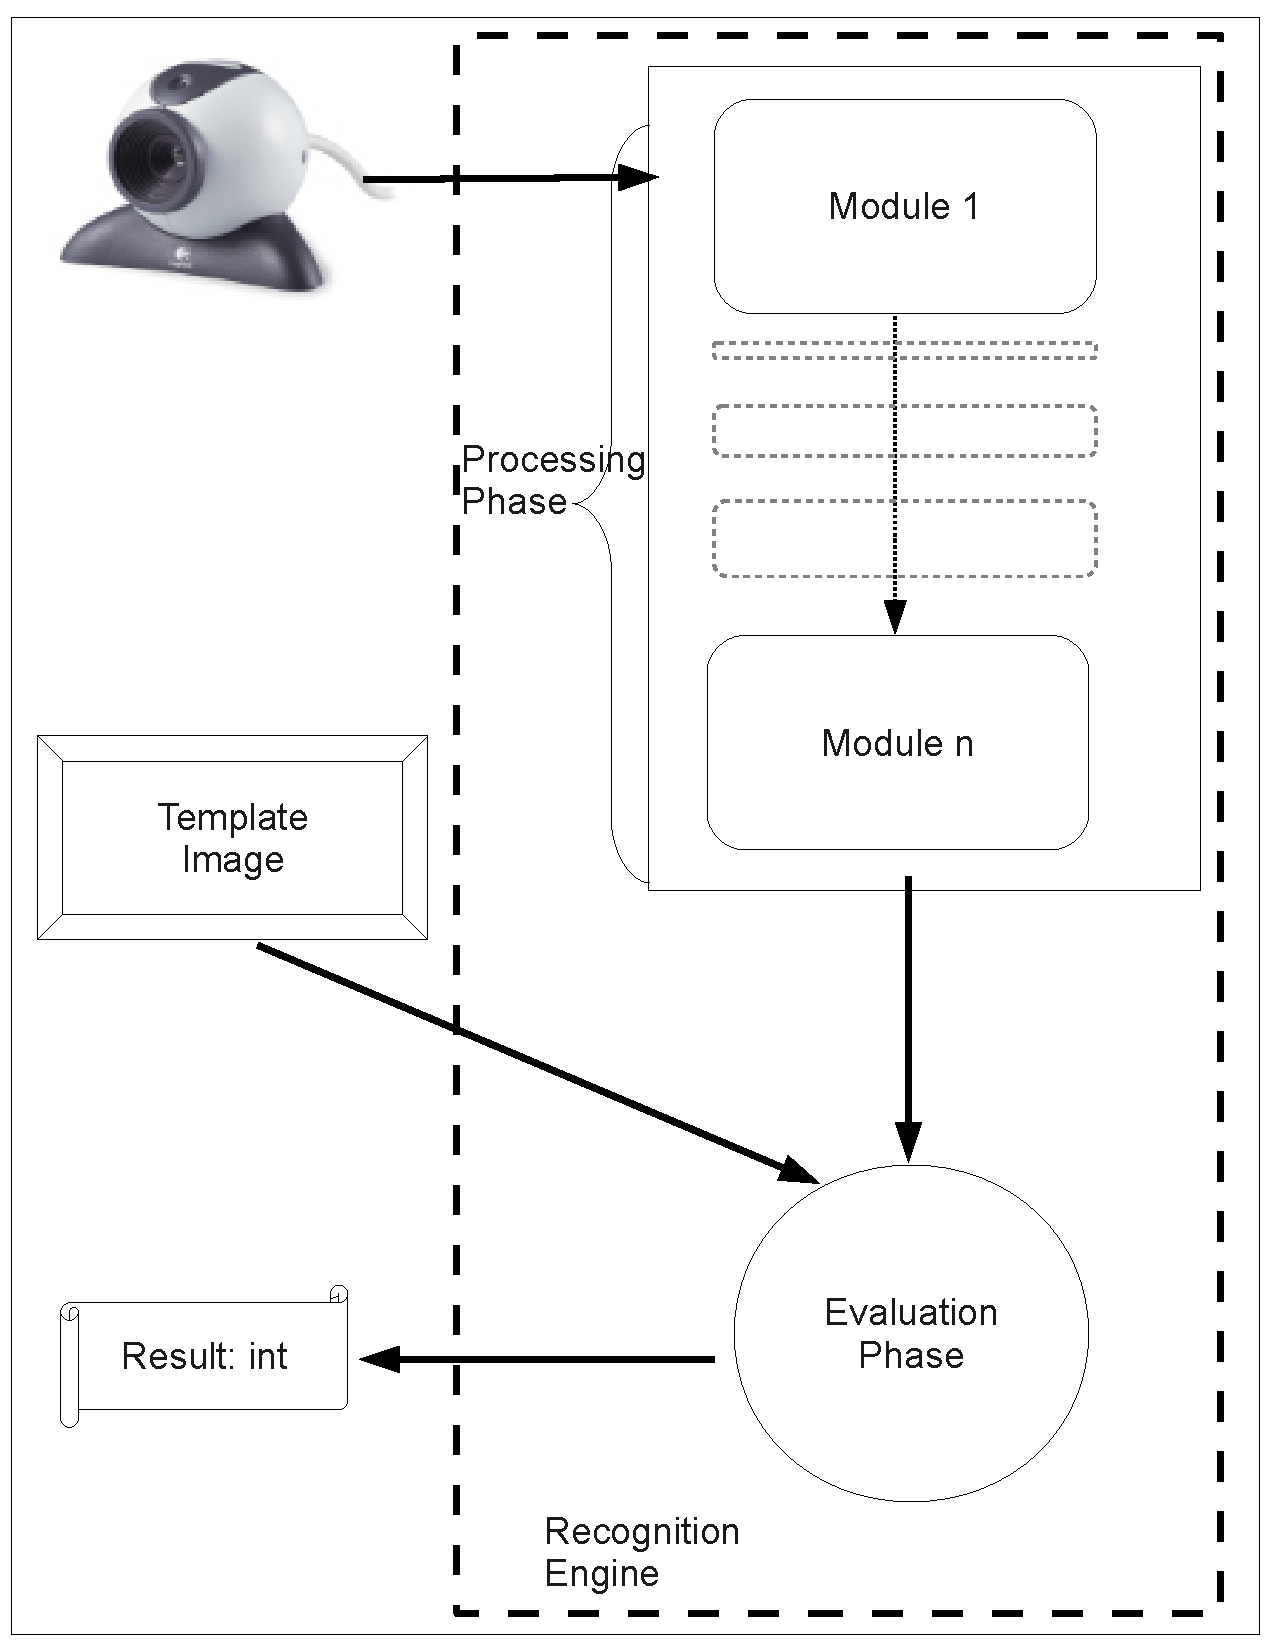
\includegraphics[scale=0.3]{recognitionEngineScheme.pdf}
    \caption{Schema del procedimento di processazione e valutazione dell'immagine in input}
    \label{reScheme}
  \end{figure}
  
  \subsubsection{L'algoritmo scelto}

  
 
\section{Alcuni Test}

\section{Osservazioni e sviluppi futuri}

\section{Coclusioni}


\clearpage

% \appendix A quick look to GOD


\nocite{*}

\bibliographystyle{plain}
\bibliography{samBibliography}

\end{document}